\chapter{Segnali e Sistemi a Tempo Discreto}

\section{Segnali a Tempo Discreto}

I segnali a tempo discreto sono rappresentati come $x[n]$, dove $n$ è un numero intero che indica l'indice temporale.

\subsection*{Esempi di segnali a tempo discreto}

\begin{itemize}
    \item \textbf{Impulso unitario} $\delta[n]$: 
    \begin{itemize}
        \item $\delta[n]=1$ se $n = 0$, altrimenti $\delta[n]=0$
        \item Da non confondere con la delta di Dirac
    \end{itemize}
    \item \textbf{Gradino unitario}:
    \begin{itemize}
        \item $u[n]=1$ per $n\geq0$, altrimenti $u[n] = 0$
    \end{itemize}
    \item \textbf{Sequenza esponenziale}:
    \begin{itemize}
        \item $x[n]= Ca^n$, dove $C$ e $a$ sono costanti
        \item Se $a$ è reale $\Rightarrow$ sequenza esponenziale reale
        \item Se $a$ è complesso $\Rightarrow$ sequenza esponenziale complessa
        \item \textbf{Sequenze unilaterali}:
        \begin{itemize}
            \item $x[n]= ca^n u[n]$ (destra)
            \item $x[n]= ca^n u[-n]$ (sinistra)
        \end{itemize}
        \item \textbf{Sequenza a singola frequenza}: $x[n]= ce^{j\omega_0 n}$
        \item \textbf{Segnale sinusoidale}: $x[n]=A\cos(\omega_0n+\varphi)$
    \end{itemize}
\end{itemize}

\section{Domini di Trasformazione}

\subsection*{Trasformata Zeta}
\begin{itemize}
    \item Definizione: $X(z)=\sum\limits_{n=-\infty}^{+\infty} x[n]z^{-n}$
    \item La somma converge solo in una \textbf{Regione di Convergenza (ROC)}
    \item La ROC è fondamentale per:
    \begin{enumerate}
        \item Inversione della trasformata Zeta
        \item Proprietà di causalità e stabilità dei sistemi
    \end{enumerate}
    \item Esempio: $X(z)=\sum\limits_{n=0}^{\infty} a^n z^{-n} \Rightarrow$ converge se $|z| > |a|$
\end{itemize}

\subsection*{Trasformata di Fourier}

\begin{itemize}
    \item Definizione: $X(e^{j\omega})=\sum\limits_{n=-\infty}^{+\infty} x[n]e^{-j\omega n}$
    \item Proprietà: periodica con periodo $2\pi$
    \item Esiste se la ROC della trasformata Z include il cerchio unitario
\end{itemize}

\subsection*{Legame tra Trasformata Z e Fourier}

\begin{itemize}
    \item Relazione: $X(z)|_{z=e^{j\omega}} = X(e^{j\omega})$
\end{itemize}

\section{Sistemi a Tempo Discreto}

\subsection*{Definizione}

Sistemi che operano su $x[n]$ per generare $y[n]$.

\subsection*{Proprietà}
\begin{itemize}
    \item \textbf{Linearità}: somma ponderata delle risposte
    \item \textbf{Stazionarietà (invarianza temporale)}
    \item \textbf{Causalità}: $y[n]$ dipende solo da $x[k]$ con $k\leq n$
    \item \textbf{Stabilità BIBO}: $\sum |h[n]| < \infty$
\end{itemize}

\subsection*{Sistemi LTI (Lineari e Tempo-Invarianti)}

\begin{itemize}
    \item \textbf{Risposta all'impulso} $h[n]$
    \item \textbf{Convoluzione}: $y[n] = \sum\limits_{m=-\infty}^{+\infty} h[m]x[n-m]$
    \item \textbf{Trasformata Z}: $Y(z)=H(z)X(z)$
\end{itemize}

\section{Sistemi a Tempo Continuo}

\subsection*{Trasformata di Fourier}
\begin{itemize}
    \item Definizione: $X(j\Omega)=\int_{-\infty}^{+\infty} x(t)e^{-j\Omega t} dt$
    \item Inversa: $x(t)=\frac{1}{2\pi} \int_{-\infty}^{+\infty} X(j\Omega)e^{j\Omega t} d\Omega$
\end{itemize}

\subsection*{Trasformata di Laplace}
\begin{itemize}
    \item Definizione: $H_a(s)=\int_{-\infty}^{+\infty} h_a(t)e^{-st} dt$
    \item Il sistema è BIBO stabile se tutti i poli sono nel semipiano sinistro: $\text{Re}[s] < 0$
\end{itemize}

\subsection*{Campionamento}

\begin{itemize}
    \item Relazione: $x[n] = x_a(nT)$ con $T>0$
    \item Aliasing se $f_s < 2f_{\text{max}}$
\end{itemize}

\section{Sistemi MIMO}

\begin{itemize}
    \item Matrice di trasferimento $H_{km}(z)$
    \item Modello: $Y(z) = H(z)U(z)$
\end{itemize}

\section{Sistemi LTI: FIR e IIR}

\subsection*{FIR (Finite Impulse Response)}

\begin{itemize}
    \item \textbf{Definizione:}
    
    \[
    H[z] = \sum_{n=0}^{N} h(n) z^{-n}
    \]
    
    dove $N+1$ è la lunghezza del filtro.
    
    \item \textbf{Stabilità:} sempre stabile se $|h(n)| < +\infty$
\end{itemize}

\subsection*{IIR (Infinite Impulse Response)}

\begin{itemize}
    \item \textbf{Definizione:} sistema non FIR
    \item \textbf{Stabilità:} può essere instabile se i poli non sono all'interno del cerchio unitario
\end{itemize}

\subsection*{Strutture per filtri razionali}

Possono essere rappresentati da funzioni razionali:
\section{Sistemi LTI: FIR e IIR}

\subsection*{Strutture per filtri razionali}

Possono essere rappresentati da funzioni razionali:

\[
H(z) = \frac{B(z)}{A(z)}
\]

\[
B(z) = \sum_{n=0}^{N} b_n z^{-n} \quad \text{e} \quad A(z) = \sum_{n=0}^{N} a_n z^{-n}
\]

\textit{Per il filtro FIR} \( A(z) = 1 \).

H(z) può essere descritta da un'equazione alle differenze della forma:

\[
a_0 y(n) = - \sum_{m=1}^{N} a_m y(n-m) + \sum_{m=0}^{N} b_m x(n-m)
\]
\textbf{Forma diretta IIR:}
\begin{figure}[H]
    \centering
    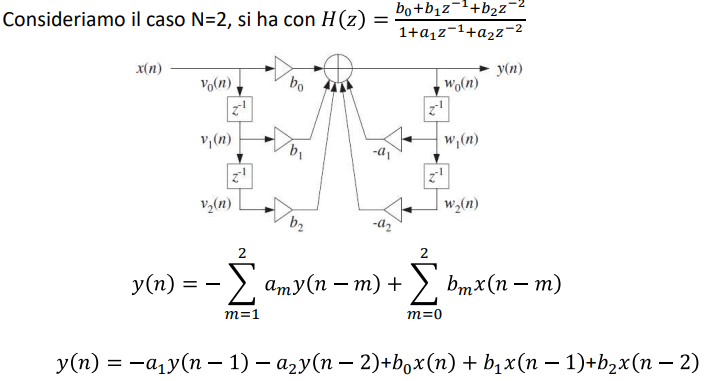
\includegraphics[width=0.7\textwidth]{capitoli/capitolo4/immagini/image1.png}
\end{figure}

\textbf{L'equazione alle differenze} può essere scritta come:

\[
w_0(n) = - a_1 w_1(n) - a_2 w_2(n) + b_0 v_0(n) + b_1 v_1(n) + b_2 v_2(n)
\]

\[
y(n) = w_n(n)
\]
\section{Forma canonica o diretta II (IIR)}

L'equazione della forma canonica diretta II è:

\[
y(n) = (b_0 x(n) + b_1 x(n-1) + b_2 x(n-2)) + (-a_1 y(n-1) - a_2 y(n-2))
\]

Dal momento che le linee di ritardo sono le stesse, non è necessario tenerle separate.
\section{Forma in cascata (IIR)}

\subsection*{Definizione}

La funzione di trasferimento viene espressa come **prodotto di sezioni del secondo ordine (SOS)**:

\[
H(z) = \prod_{i=0}^{K-1} H_i(z)
\]

con ogni \( H_i(z) \) rappresentante una sezione del secondo ordine.

Ogni **funzione di trasferimento razionale** può essere riscritta come prodotto di sezioni del secondo ordine:

\[
H(z) = \frac{b_0 + b_1 z^{-1} + b_2 z^{-2} + \dots + b_M z^{-M}}{1 + a_1 z^{-1} + a_2 z^{-2} + \dots + a_N z^{-N}}
\]

\subsection*{Struttura della Forma in Cascata}

- Ogni **sezione** può essere implementata con una **forma canonica diretta** (o trasposta).
- Convenzionalmente, si utilizza **la forma canonica**.

\subsection*{Segnali di ingresso e uscita}

- **Ingresso del sistema**: il segnale \( x(n) \) entra nella prima sezione.
- **Uscita del sistema**: il segnale in uscita dall'ultima sezione \( y(n) \).
- **Per gli step intermedi**: l’uscita della sezione \( i \) è l’ingresso della sezione \( i+1 \).

\subsection*{Vettore di stato di ogni sezione}

Ogni sezione ha uno **stato interno**:

\[
s_i = [s_{i0}, s_{i1}, s_{i2}]
\]

che rappresenta i **ritardi interni** della sezione.

\subsection*{Equazione alle differenze}

Deriva dalla **forma canonica del secondo ordine**, iterata per tutte le sezioni:

\[
y(n) = -a_1 y(n-1) - a_2 y(n-2) + b_0 x(n) + b_1 x(n-1) + b_2 x(n-2)
\]

\subsection*{Pseudocodice per il calcolo sequenziale}

\[
\begin{aligned}
    x_0 &= x(n) \\
    y_i &= \sum (\text{contributo ritardi e coefficienti}) \\
    x_{i+1} &= y_i \\
    y(n) &= y_{K-1}
\end{aligned}
\]


\section{Assaggio da Forma Diretta/Canonica a Cascata}

La conversione da una **forma diretta** (o canonica) a una **forma in cascata** segue questi passaggi fondamentali:

\begin{enumerate}
    \item **Fattorizzazione** del numeratore e del denominatore nei **polinomi del secondo ordine**.
    \item **Trovare le radici** dei due polinomi.
    \item **Raggruppare in polinomi quadratici**:
    \begin{itemize}
        \item Se \textbf{radici reali}:
        \[
        (1 - \alpha_1 z^{-1} + \alpha_2 z^{-2})
        \]
        \item Se \textbf{radici complesse coniugate}:
        \[
        (1 - \beta_1 z^{-1} + \beta_2 z^{-2})
        \]
    \end{itemize}
\end{enumerate}

Questa forma a cascata è utile per garantire una maggiore **stabilità numerica** e per facilitare l’implementazione pratica dei filtri IIR.

\textbf{Forma diretta FIR:}
\begin{figure}[H]
    \centering
    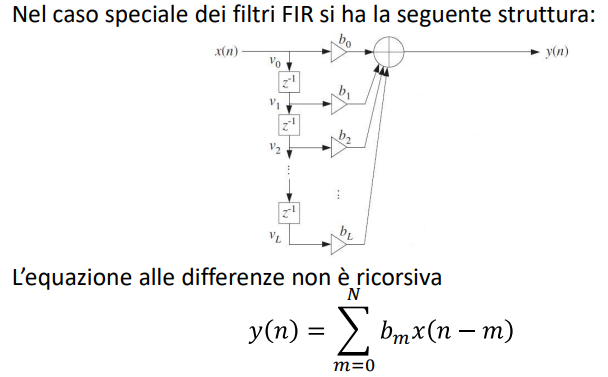
\includegraphics[width=0.7\textwidth]{capitoli/capitolo4/immagini/image2.png}
\end{figure}

\section{Tecniche di filtraggio per filtri IIR}

\subsection{Funzioni delle Librerie Intel}
\begin{itemize}
    \item \textit{Implementazione} suddivisa in:
    \begin{enumerate}
        \item \textbf{Inizializzazione} del filtro
        \item \textbf{Esecuzione del filtraggio}
    \end{enumerate}
    \item Due tipi di \textit{filtri} supportati:
    \begin{enumerate}
        \item \textbf{Filtri di ordine arbitrario} → implementati in \textbf{forma diretta}
        \item \textbf{Filtri biquad} → implementati in \textbf{forma a cascata} (sezioni del secondo ordine)
    \end{enumerate}
\end{itemize}

\subsection{Esempio NU-Tech}
\begin{itemize}
    \item \textbf{Struttura del filtro} dipende dal tipo scelto
    \item \textbf{Inizializzazione richiesta} prima di applicare il filtro
    \item \textbf{Struttura} \texttt{ctx}:
    \begin{itemize}
        \item Contiene i coefficienti \textbf{B} seguiti dai coefficienti \textbf{A} (taps)
    \end{itemize}
\end{itemize}

\subsection{Due Approcci Principali}
\begin{enumerate}
    \item Filtraggio campione per campione (\textbf{Forma Diretta})
    \item Filtraggio a blocchi (\textbf{per segnali lunghi})
\end{enumerate}

\subsection{Forma Diretta e Convoluzione}
Per i sistemi \textbf{LTI}, il filtraggio FIR si basa sulla \textbf{convoluzione}:
\[
    y(n) = \sum_{m=0}^{M} h(m)x(n-m)
\]

\noindent Espressione compatta:
\begin{itemize}
    \item La \textbf{lunghezza finale} del segnale filtrato sarà \(L + M - 1\)
    \item Si basa sul \textbf{concetto di scorrimento} del segnale di input sulla risposta all’impulso
\end{itemize}

\subsection{Funzioni delle Librerie Intel}
\begin{itemize}
    \item Funzione di \textbf{convoluzione} (simile a \texttt{conv} di MATLAB)
    \item Funzioni di \textbf{filtraggio FIR} (inizializzazione come per i filtri IIR, simile a \texttt{filter} di MATLAB)
\end{itemize}

\subsection*{Convoluzione a Blocchi}

La convoluzione a blocchi è utilizzata per il filtraggio real-time di segnali di lunghezza infinita con filtri FIR. Costituisce la base di molte applicazioni in tempo reale.

\medskip

Sono disponibili diversi approcci:

\begin{itemize}
    \item \textbf{OLS (Overlap and Save)}: ad ogni aggiornamento si effettua uno shift del vettore di ingresso verso sinistra, mantenendo solo la parte utile dell'IFFT.
    \item \textbf{OLA (Overlap and Add)}: ad ogni aggiornamento si somma il blocco corrente con quello precedente, dopo aver effettuato uno shift a sinistra.
    \item \textbf{Versione Partizionata}: adatta per blocchi più piccoli (\(L_{\text{BLOCK}} < L_H\)), suddivide il filtro in più blocchi.
\end{itemize}
\textbf{Confronto tra i metodi:}

\begin{table}[H]
\centering
\begin{tabularx}{\textwidth}{|X|X|X|X|}
\hline
\textbf{Metodo} & \textbf{Principio} & \textbf{Vantaggi} & \textbf{Svantaggi} \\
\hline
\textbf{OLS (Overlap and Save)} & Mantiene solo la parte utile dell'IFFT & Risparmio di memoria & Possibile aliasing se non implementato correttamente \\
\hline
\textbf{OLA (Overlap and Add)} & Somma delle finestre successive & Maggiore fedeltà del segnale & Richiede gestione accurata dell'overlap \\
\hline
\textbf{Partizionata} & Suddivide il filtro in blocchi più piccoli & Più efficiente per filtri lunghi & Implementazione più complessa \\
\hline
\end{tabularx}
\caption{Confronto tra approcci per la convoluzione a blocchi}
\end{table}

\section{Convoluzione a Blocchi: OLS (Overlap and Save)}

\textbf{Passaggi principali:}

\begin{enumerate}
    \item \textbf{Shift del buffer} (spostamento di $fs$ campioni)
    \begin{verbatim}
    ippsMove_64f(buffOls + fs, buffOls, fs);
    \end{verbatim}
    
    \item \textbf{Copia dei nuovi $fs$ campioni in fondo al buffer}
    \begin{verbatim}
    ippsCopy_64f((double*)(*Input[0]).DataBuffer, buffOls + fs, fs);
    \end{verbatim}
    
    \item \textbf{Trasformata di Fourier del buffer ($buffOls \to buffOlsF$)}
    \begin{verbatim}
    ippsFFTFwd_RToPack_64f(buffOls, buffOlsF, fftState, 0);
    \end{verbatim}
    
    \item \textbf{FFT dei coefficienti del filtro ($taps \to tapsF$)}
    \begin{verbatim}
    ippsFFTFwd_RToPack_64f_I(tapsF, fftState, 0);
    \end{verbatim}
    
    \item \textbf{Moltiplicazione in frequenza ($buffOlsF \cdot tapsF$)}
    \begin{verbatim}
    ippsMulPack_64f_I(tapsF, buffOlsF, 2fs);
    \end{verbatim}
    
    \item \textbf{Trasformata inversa di Fourier (IFFT)}
    \begin{verbatim}
    ippsFFTInv_PackToR_64f_I(buffOlsF, fftState, 0);
    \end{verbatim}
    
    \item \textbf{Aggiornamento dell'output} (estrazione dei campioni validi)
    \begin{verbatim}
    ippsCopy_64f(buffOlsF + fs, (double*)(*Output[0]).DataBuffer, fs);
    \end{verbatim}
\end{enumerate}

\vspace{3cm}

\section{Convoluzione a Blocchi Partizionata}

\textbf{Passaggi principali:}

\begin{enumerate}
    \item \textbf{Inizializzazione del frame}
    \begin{verbatim}
    CBFunction(this, NUTS_GETFRAME_RATE, 0, &ActualFrameSize);
    in_ols = new double[2*ActualFrameSize];
    memset(in_ols, 0.0, 2*ActualFrameSize * sizeof(double));
    \end{verbatim}
    
    \item \textbf{Copia dei dati di input nel buffer $in\_ols$ e calcolo FFT}
    \begin{verbatim}
    ippsCopy_64f((double*)Input[0]->DataBuffer, in_ols, FrameSize);
    ippsFFTFwd_RToPerm_64f(in_ols, TmpFreqRis, IPP_Spec, NULL);
    \end{verbatim}
    
    \item \textbf{Loop sulla partizione dei coefficienti del filtro}
    \begin{verbatim}
    for(int j = 0; j < ceil(len_taps / FrameSize); j++) {
    ippsCopy_64f(taps + j * FrameSize, taps_cut, FrameSize);
    ippsFFTFwd_RToPerm_64f(taps_cut, fft_taps, IPP_Spec, NULL);
    ippsMulPerm_64f_I(TmpFreqRis, fft_taps, 2 * FrameSize);
    ippsFFTInv_PermToR_64f_I(fft_taps, IPP_Spec, NULL);
    }
    \end{verbatim}
    
    \item \textbf{Gestione del delay per la sovrapposizione delle partizioni}
    \begin{verbatim}
    ippsCopy_64f(fft_taps, delay + j * FrameSize, FrameSize);
    memset(taps_cut, 0.0, FrameSize * sizeof(double));
    memset(fft_taps, 0.0, FrameSize * sizeof(double));
    \end{verbatim}
    
    \item \textbf{Somma con il buffer precedente e aggiornamento dell'output}
    \begin{verbatim}
    ippsAdd_64f_I(delay_old, delay, len_delay_old);
    ippsCopy_64f(delay, (double*)Output[0]->DataBuffer, FrameSize);
    ippsCopy_64f(delay + FrameSize, delay_old, len_delay_old);
    \end{verbatim}
\end{enumerate}




